
%(BEGIN_QUESTION)
% Copyright 2010, Tony R. Kuphaldt, released under the Creative Commons Attribution License (v 1.0)
% This means you may do almost anything with this work of mine, so long as you give me proper credit

A PLC is being used to monitor the oil pressure for a steam turbine driving an electrical generator, shutting steam off to the turbine if ever the oil pressure drops below a 10 PSI limit.  The turbine's lubrication oil pump is driven by the turbine shaft itself, supplying itself with pressurized lubricating oil to keep all the turbine bearings properly lubricated and cooled:

$$\includegraphics[width=15.5cm]{i00189x01.eps}$$

\vskip 10pt

Another technician programmed the PLC for the start/stop function, but this program has a problem:

$$\includegraphics[width=15.5cm]{i00189x02.eps}$$

Identify what this problem is, and fix it!  Hint: the oil pump is driven by the turbine, and as such cannot generate any oil pressure until the turbine begins to spin.

\underbar{file i00189}
%(END_QUESTION)





%(BEGIN_ANSWER)

This is one possible fix for the problem:

$$\includegraphics[width=15.5cm]{i00189x03.eps}$$

%(END_ANSWER)





%(BEGIN_NOTES)

The problem is the turbine can never start up, due to a Catch-22: the solenoid valve will never be allowed to energize (to send steam to the turbine) unless the oil pressure permissive contact closes.  However, this contact cannot close unless there is adequate oil pressure output by the pump, which cannot happen until the turbine begins to spin!

In the proposed solution, the operator must hold the ``Start'' pushbutton long enough for the turbine to gain enough speed to build adequate oil pressure.  Only then will the system ``latch'' in the run mode.










\vfil \eject

\noindent
{\bf Prep Quiz:}

Identify one plausible fault to explain why this PLC-controlled motor refuses to start up when the ``Start'' button is pressed, given the following wiring diagram and online PLC program display shown below.  Note: no one is pushing any buttons at this time.

$$\includegraphics[width=15.5cm]{i00189x04.eps}$$






\vfil \eject

\noindent
{\bf Prep Quiz:}

Identify one plausible fault to explain why this PLC-controlled motor refuses to start up when the ``Start'' button is pressed, given the following wiring diagram and online PLC program display shown below.  Note: no one is pushing any buttons at this time.

$$\includegraphics[width=15.5cm]{i00189x05.eps}$$






\vfil \eject

\noindent
{\bf Prep Quiz:}

Identify one plausible fault to explain why this PLC-controlled motor refuses to start up when the ``Start'' button is pressed, given the following wiring diagram and online PLC program display shown below.  Note: no one is pushing any buttons at this time.

$$\includegraphics[width=15.5cm]{i00189x06.eps}$$


%INDEX% PLC, troubleshooting: turbine lube oil shutdown control
%INDEX% Process: steam turbine auto-shutdown 

%(END_NOTES)


